\documentclass[11pt]{article}
\usepackage[margin=1in]{geometry}
\usepackage{amsmath,amssymb,amsthm,mathtools}
\usepackage{graphicx}
\usepackage{microtype}
\usepackage{xcolor}
\usepackage[hidelinks]{hyperref}
\usepackage{enumitem}

\newtheorem{theorem}{Theorem}
\newtheorem{proposition}{Proposition}
\newtheorem{corollary}{Corollary}
\newtheorem{remark}{Remark}
\newcommand{\R}{\mathbb{R}}
\newcommand{\ip}[2]{\langle #1,#2\rangle}

\title{Minimal Weak Phase Retrieval:\\
A Cofactor Characterization, an Algebraic Nullity Theorem,\\
and a Correction to the Published $\R^4$ Example}
\author{Candidate partial result for arXiv:2110.06868}
\date{17 August 2026}

\begin{document}
\maketitle

\begin{center}
\fbox{\parbox{0.91\textwidth}{\textbf{Status.}
Candidate partial result, likely valid, pending human review.  The packet gives
a full finite characterization of minimal weak phase retrieval and strengthens
Problem 9.1 from non-density to containment in a proper algebraic hypersurface,
hence nowhere density and Lebesgue nullity.  Problem 9.1 itself was already
answered in later literature.  The packet does not solve the existence question
in Problem 9.2.  It does show that the six-vector $\R^4$ example cited as
motivation for Problem 9.2 is not weak phase retrievable.}}
\end{center}

\section{Source and extracted problems}

The source is F. Akrami, P. G. Casazza, A. Rahimi,
M. A. Hasankhani Fard, and B. Daraby,
\emph{A note on (weak) phase and norm retrievable Real Hilbert space frames
and projections}, arXiv:2110.06868 \cite{AKRAMI2021}.
Section 9, page 14, asks:
\begin{quote}
\textbf{Problem 9.1.} Show that the weak phase retrievable frames with
$2n-2$ vectors in $\R^n$ are not dense in all frames with $2n-2$ vectors.
\end{quote}
The source then says that examples with $2n-2$ vectors are known for
$n=3,4$, and Problem 9.2 asks for such examples for every $n\geq 5$.

\begin{figure}[ht]
\centering
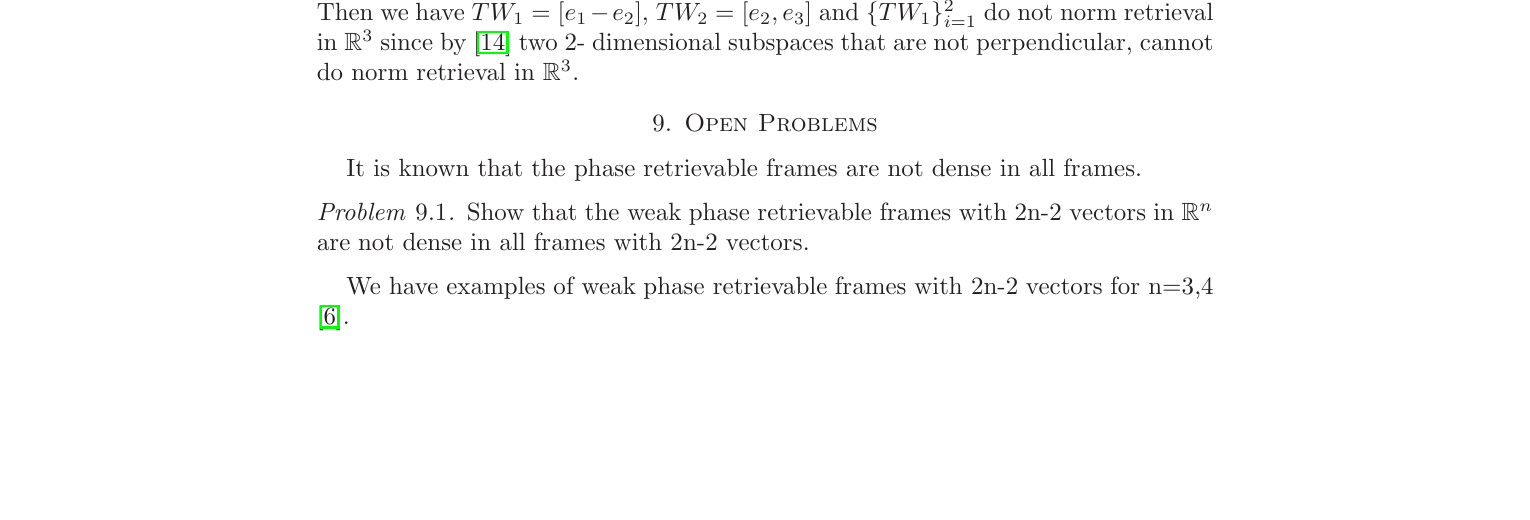
\includegraphics[width=\textwidth]{figures/open_problem_9_1_crop.png}
\caption{Problem 9.1 in the source paper, page 14.}
\end{figure}

\begin{figure}[ht]
\centering
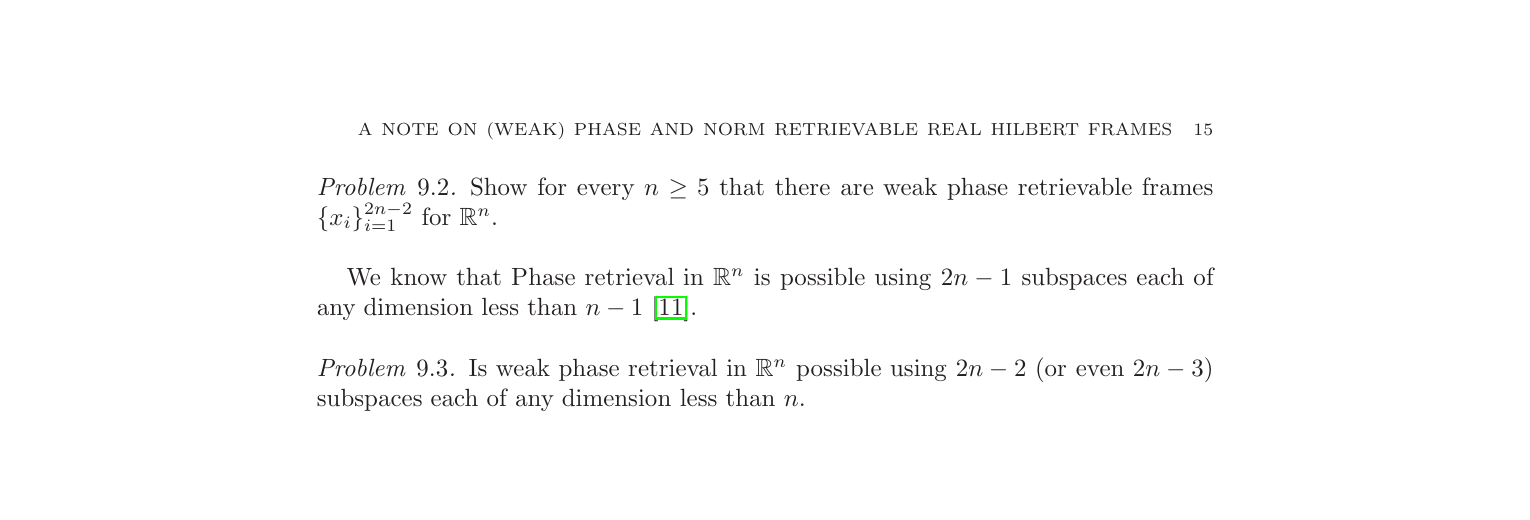
\includegraphics[width=\textwidth]{figures/open_problems_9_2_9_3_crop.png}
\caption{Problems 9.2 and 9.3 in the source paper, page 15.}
\end{figure}

\clearpage
\section{Definitions and cofactor notation}

Let $A\in\R^{(2n-2)\times n}$ have rows
$\phi_1^T,\ldots,\phi_{2n-2}^T$.  Its rows do \emph{weak phase retrieval}
if
\[
  |\ip{x}{\phi_i}|=|\ip{y}{\phi_i}|\quad(1\leq i\leq 2n-2)
\]
implies that there is $\varepsilon\in\{\pm1\}$ such that
$\operatorname{sgn}(x_j)=\varepsilon\operatorname{sgn}(y_j)$ whenever
$x_jy_j\ne0$.  The matrix is \emph{full spark} if every $n$ rows are
linearly independent.

For $I\subset[2n-2]$ with $|I|=n-1$, let $A_I$ be the corresponding row
submatrix and define its signed cofactor vector
\[
 c_I(A)_j=(-1)^{j-1}\det A_{I,[n]\setminus\{j\}},\qquad 1\leq j\leq n.
\]
Then $A_Ic_I(A)=0$.  Put
\[
 S_I(A)=\sum_{j=1}^n c_I(A)_j^2.
\]
If $A$ is full spark, every $A_I$ has rank $n-1$, so $S_I(A)>0$.

\section{Proof intuition}

Every nontrivial magnitude ambiguity of a full-spark $(2n-2)$-row matrix
comes from a balanced partition $I\sqcup I^c$ of its rows.  The difference
and sum of the two ambiguous signals lie on the two kernel lines
$\ker A_I$ and $\ker A_{I^c}$.  Weak phase retrieval holds exactly when the
unit vectors on those two lines have equal absolute value in every coordinate.
Cofactor vectors give polynomial coordinates for the kernel lines, turning
this geometric criterion into finitely many determinant equations.

For non-density, only one balanced partition is needed.  Weak phase retrieval
forces one explicit cofactor polynomial to vanish, while a simple pair of
shifted coordinate blocks makes that polynomial equal to one.  The weak phase
retrievable locus therefore lies in the zero set of a nonzero polynomial.

\section{Finite cofactor characterization}

\begin{theorem}[Cofactor characterization]\label{thm:characterization}
Let $n\geq2$ and $A\in\R^{(2n-2)\times n}$.  The rows of $A$ do weak phase
retrieval if and only if both of the following hold:
\begin{enumerate}[label=(\roman*)]
\item $A$ is full spark;
\item for every $I\subset[2n-2]$ with $|I|=n-1$ and every $j\in[n]$,
\begin{equation}\label{eq:cofactor}
 c_I(A)_j^2 S_{I^c}(A)=c_{I^c}(A)_j^2 S_I(A).
\end{equation}
\end{enumerate}
Equivalently, the normalized kernel generators of $A_I$ and $A_{I^c}$
have identical coordinatewise absolute values for every balanced partition.
\end{theorem}

\begin{proof}
Suppose first that the rows do weak phase retrieval.  A known minimal-cardinality
theorem says that a weak phase retrievable family of $2n-2$ vectors in $\R^n$
is full spark \cite[Theorem 3.7]{BOTELHO2016}.  Fix a balanced partition and set
\[
 u=\frac{c_I(A)}{\sqrt{S_I(A)}},\qquad
 v=\frac{c_{I^c}(A)}{\sqrt{S_{I^c}(A)}}.
\]
For $i\in I$, $u$ is orthogonal to $\phi_i$, while for $i\in I^c$, $v$ is
orthogonal to $\phi_i$.  Consequently
\[
 |\ip{u+v}{\phi_i}|=|\ip{u-v}{\phi_i}|\qquad(1\leq i\leq2n-2).
\]
Weak phase retrieval says that all nonzero products
$(u_j+v_j)(u_j-v_j)=u_j^2-v_j^2$ have one common sign, up to reversing all
signs.  But
\[
 \sum_{j=1}^n(u_j^2-v_j^2)=\|u\|^2-\|v\|^2=0.
\]
Thus every term is zero: $u_j^2=v_j^2$ for all $j$.  Clearing denominators
gives \eqref{eq:cofactor}.

Conversely, assume (i) and (ii), and suppose $x,y\in\R^n$ give the same
measurement magnitudes.  For each row choose a sign so that
$\ip{x}{\phi_i}=\pm\ip{y}{\phi_i}$, assigning an arbitrary sign if both
inner products vanish.  Let $I$ be the plus-sign indices.  Then
\[
 A_I(x-y)=0,\qquad A_{I^c}(x+y)=0.
\]
If $|I|\geq n$, full spark gives $x=y$; if $|I^c|\geq n$, it gives $x=-y$.
The only other possibility is $|I|=|I^c|=n-1$.

In the balanced case, there are scalars $a,b$ such that
\[
 x-y=au,\qquad x+y=bv,
\]
where $u$ and $v$ are the normalized cofactor vectors above.  Condition (ii)
provides signs $d_j\in\{\pm1\}$, arbitrary when $u_j=v_j=0$, with
$v_j=d_ju_j$.  Hence
\[
 x_jy_j=\frac{(bv_j+au_j)(bv_j-au_j)}{4}
        =\frac{b^2-a^2}{4}u_j^2.
\]
All nonzero coordinate products therefore have the same sign.  This is exactly
weak equality or weak opposition of phase, proving the converse.
\end{proof}

\section{Algebraic strengthening of Problem 9.1}

\begin{corollary}[Proper algebraic locus]\label{cor:null}
For every $n\geq2$, the set of weak phase retrievable
$(2n-2)$-element families in $\R^n$ is contained in a proper real-algebraic
hypersurface of $\R^{(2n-2)n}$.  In particular, it is nowhere dense and has
Lebesgue measure zero.
\end{corollary}

\begin{proof}
Fix $I_0=\{1,\ldots,n-1\}$ and define the polynomial
\[
 F(A)=c_{I_0}(A)_n^2S_{I_0^c}(A)
      -c_{I_0^c}(A)_n^2S_{I_0}(A).
\]
Theorem \ref{thm:characterization} gives $F(A)=0$ for every weak phase
retrievable $A$.

This polynomial is not identically zero.  Let the first $n-1$ rows of $A_0$
be $e_1^T,\ldots,e_{n-1}^T$ and the last $n-1$ rows be
$e_2^T,\ldots,e_n^T$.  Up to irrelevant signs,
$c_{I_0}(A_0)=e_n$ and $c_{I_0^c}(A_0)=e_1$, so $F(A_0)=1$.
The zero set of a nonzero real polynomial is closed, has empty interior, and
has Lebesgue measure zero.  It contains the weak phase retrievable locus and
its closure, proving the claim.
\end{proof}

Casazza and Akrami later proved the non-density requested in Problem 9.1 for
all $m\geq2n-2$ \cite[Theorem 6]{CASAZZA2023}.  Corollary
\ref{cor:null} is an independent strengthening for the minimal case: it gives
an explicit algebraic certificate and measure-zero conclusion.

\section{The published $\R^4$ example fails}

The $n=4$ example cited in the source comes from
Botelho-Andrade, Casazza, Ghoreishi, Jose, and Tremain
\cite[p.~12]{BOTELHO2016}.  Its measurement rows are
\[
 \Phi=\begin{bmatrix}
 1&1&1&-1\\
 -1&1&1&1\\
 1&-1&1&1\\
 1&1&-1&-1\\
 1&-1&1&-1\\
 1&-1&-1&1
 \end{bmatrix}.
\]

\begin{figure}[ht]
\centering
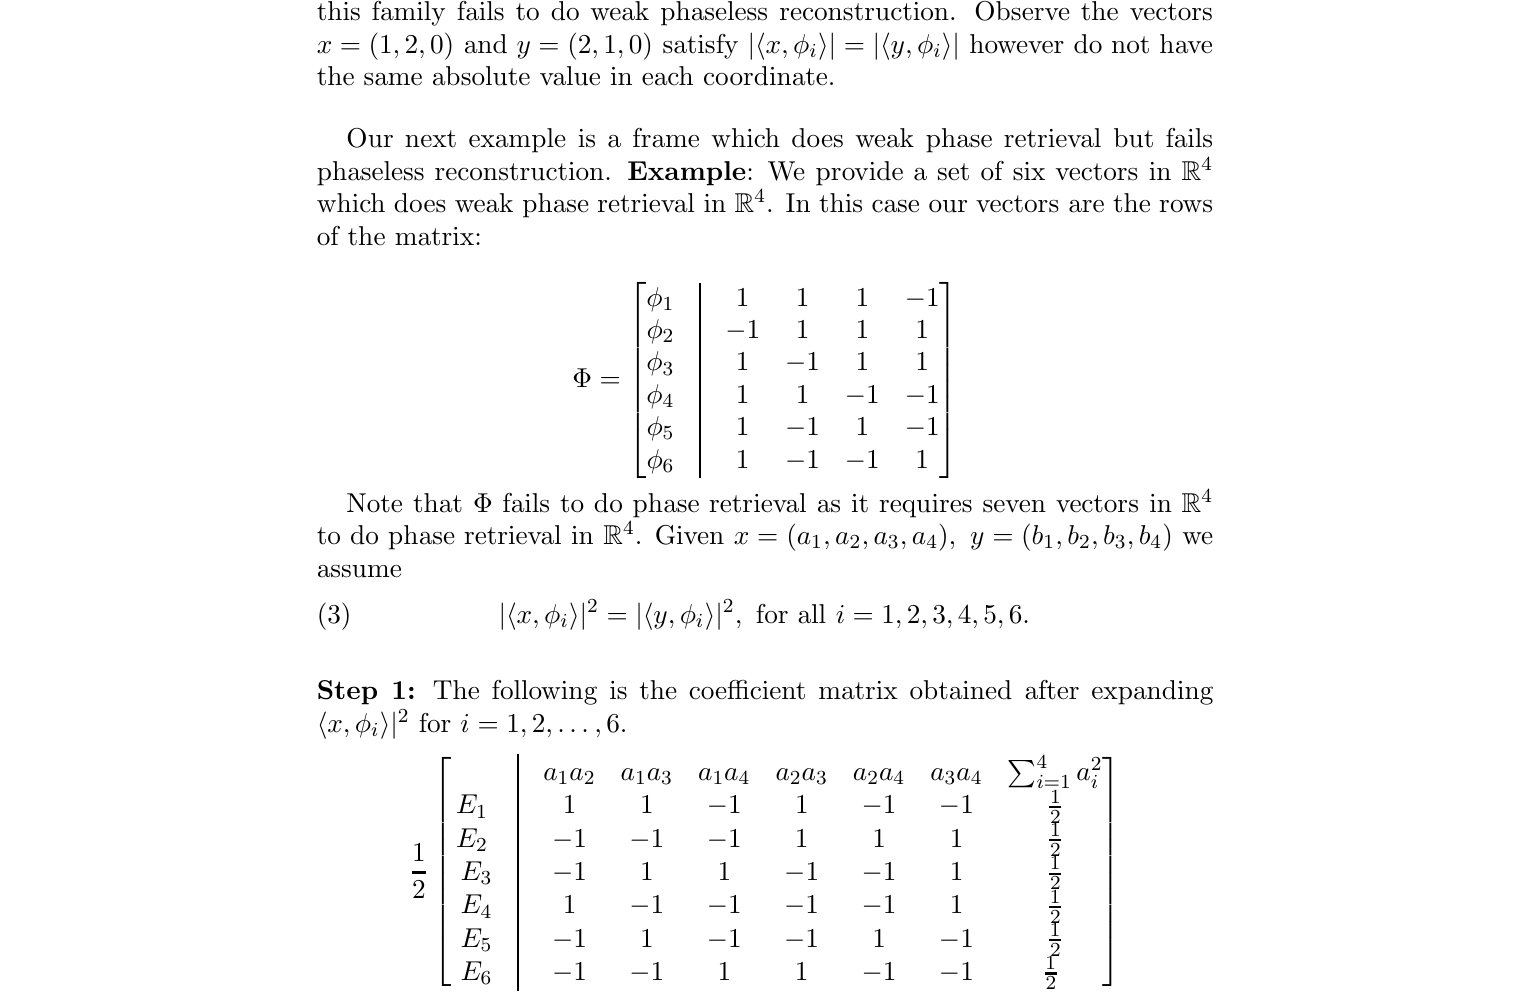
\includegraphics[width=\textwidth]{figures/published_n4_example_crop.png}
\caption{The claimed six-vector $\R^4$ example in arXiv:1612.08018, page 12.}
\end{figure}

\begin{proposition}\label{prop:badexample}
The rows of $\Phi$ do not weak phase retrieval in $\R^4$.
\end{proposition}

\begin{proof}
Take
\[
 x=(2,1,0,1),\qquad y=(0,-1,0,1).
\]
Direct multiplication gives
\[
 |\Phi x|=|\Phi y|=(2,0,2,2,0,2)^T.
\]
On the two coordinates where both vectors are nonzero,
$x_2y_2=-1$ while $x_4y_4=1$.  Thus $x$ and $y$ have neither weakly the same
nor weakly opposite signs.  This violates weak phase retrieval.

There is also an immediate consistency check: the first, second, fourth, and
fifth rows satisfy
\[
 -\phi_1+\phi_2+\phi_4+\phi_5=0.
\]
Hence $\Phi$ is not full spark, contrary to the necessary full-spark theorem
for a six-vector weak phase retrievable family in $\R^4$.
\end{proof}

The explicit pair in Proposition \ref{prop:badexample} is decisive and does
not depend on diagnosing any particular step of the published row reduction.
It means that the sentence preceding Problem 9.2 should not cite this matrix
as a verified $n=4$ example.  This packet does not prove that no other
six-vector example in $\R^4$ exists.

\section{Computational verification and bounded searches}

The reusable exact checker in \texttt{code/verify\_cofactor\_theorem.py}:
\begin{itemize}
\item verifies full spark and every cofactor equation for the published
$n=3$ example;
\item verifies the equal-magnitude counterexample to the published $n=4$
matrix;
\item checks $F(A_0)=1$ exactly for $2\leq n\leq8$.
\end{itemize}
Run it from the packet directory with
\begin{verbatim}
conda run --no-capture-output -n sandbox python \
  code/verify_cofactor_theorem.py
\end{verbatim}
All checks pass using integer arithmetic.  The symbolic proof above, not this
finite check, establishes the theorem for every $n$.

The separate exact script \texttt{code/search\_sign\_frames\_n5.py} exhausts
all $\binom{16}{8}=12{,}870$ projective choices of eight $\{\pm1\}$ rows in
$\R^5$.  None is full spark.  This rules out only the direct sign-vector
extension of the $n=3$ construction; it is not evidence sufficient to settle
Problem 9.2.

\section{Limitations and novelty check}

Problem 9.2 (existence for $n\geq5$) and Problem 9.3 (retrieval by fewer
subspaces) remain open in this packet.  Numerical searches in $n=4,5$ repeatedly
approached the cofactor equations only by collapsing a coordinate or losing a
minor.  Those observations are recorded in the attempt log and are not used as
proof.

The bounded novelty audit searched the run's parsed arXiv corpus, cheap result
indexes, and current arXiv/web results for combinations of
``weak phase retrieval'' with ``cofactor'', ``algebraic variety'',
``measure zero'', ``Lebesgue null'', and ``nowhere dense''.  It directly
inspected arXiv:1612.08018, 2110.06868, 2301.03520, and 2301.05045.  The search
found the later non-density theorem \cite{CASAZZA2023}, but no cofactor
characterization, algebraic-nullity strengthening, or published correction of
the six-vector $\R^4$ matrix.  Novelty confidence is moderate rather than
definitive because this was a bounded search, not a complete citation review.

\section{Human-review recommendation}

Review is recommended, with priority on three short points:
\begin{enumerate}
\item the sufficiency direction of Theorem \ref{thm:characterization},
especially the balanced partition case;
\item the nonzero-polynomial witness in Corollary \ref{cor:null};
\item the direct multiplication in Proposition \ref{prop:badexample}.
\end{enumerate}
If these pass, the characterization and algebraic-nullity theorem should be
treated as a likely new strengthening, while the $\R^4$ calculation should be
communicated as a correction to the motivating example rather than as a
solution of Problem 9.2.

\begin{thebibliography}{9}
\bibitem{AKRAMI2021}
F. Akrami, P. G. Casazza, A. Rahimi, M. A. Hasankhani Fard, and B. Daraby,
\emph{A note on (weak) phase and norm retrievable Real Hilbert space frames
and projections}, arXiv:2110.06868 (2021).

\bibitem{BOTELHO2016}
S. Botelho-Andrade, P. G. Casazza, D. Ghoreishi, S. Jose, and J. C. Tremain,
\emph{Weak phase retrieval and phaseless reconstruction},
arXiv:1612.08018 (2016).

\bibitem{CASAZZA2023}
P. G. Casazza and F. Akrami,
\emph{Classifying weak phase retrieval}, arXiv:2301.03520 (2023).
\end{thebibliography}

\end{document}
